\documentclass[11pt]{report}
\usepackage{fontspec}
\usepackage{polyglossia}
% Define the Hebrew-capable fonts BEFORE activating the Hebrew main language so
% polyglossia's Hebrew gloss finds \hebrewfont / \hebrewfonttt (and a Hebrew-capable
% monospace font) at load time. Without this, polyglossia raises
% "current main monospace font ... does not contain the Hebrew script" at
% \printbibliography. Adjust the family to one installed on the build machine
% (e.g. "David CLM" / "Frank Ruehl CLM" from the culmus package).
\setmainfont{David CLM}
\newfontfamily\hebrewfont{David CLM}
\newfontfamily\hebrewfonttt{David CLM}
\setmonofont{David CLM}
\newfontfamily\englishfont{Latin Modern Roman}
\setmainlanguage{hebrew}
\setotherlanguage{english}
\usepackage{amsmath}
\usepackage{graphicx}
% Compilation runs inside generated/latex/, where the renderer copies images into
% generated/latex/assets/ and references them as assets/<name>; search from cwd.
\graphicspath{{./}}
\usepackage{booktabs}
\usepackage[backend=biber]{biblatex}
\addbibresource{references.bib}
\usepackage{hyperref}
% Deliberate headers/footers (assignment 13.1): running chapter title + page number.
\usepackage{fancyhdr}
\pagestyle{fancy}
\fancyhf{}
\fancyhead[L]{\nouppercase{\leftmark}}
\fancyfoot[C]{\thepage}
\renewcommand{\headrulewidth}{0.4pt}

\title{ניתוח כדורגל מבוסס נתונים: מ-xG לאסטרטגיית משחק}
\author{Amr Safadi and Sharbel Maroun}
\date{2026-06-04}

\begin{document}
\begin{titlepage}
\centering
\vspace*{3cm}
{\Huge ניתוח כדורגל מבוסס נתונים: מ-xG לאסטרטגיית משחק\par}
\vspace{0.6cm}
{\Large כיצד AI, מדדים טקטיים וגרפים משנים החלטות של מאמנים ומועדונים\par}
\vspace{2.5cm}
{\large Amr Safadi and Sharbel Maroun\par}
\vspace{0.4cm}
{\large AI Agent Orchestration\par}
{\large מרצה: Dr. Yoram Segal\par}
\vspace{0.4cm}
{\large 2026-06-04\par}
\end{titlepage}\tableofcontents
\chapter{מהאינטואיציה של המאמן לניתוח כדורגל מבוסס נתונים}
\section{מדוע כדורגל הוא בעיית החלטה מורכבת}
כדורגל נראה לעיתים כמשחק פשוט: עשרים ושניים שחקנים, כדור אחד ושערים משני הצדדים. בפועל זהו מרחב החלטה מורכב מאוד, שבו כל פעולה קטנה משנה את האפשרויות של כל השחקנים סביב הכדור. מאמן צריך להחליט כיצד ללחוץ, איפה להציב את קו ההגנה, מתי לשנות מערך, ואילו שחקנים מתאימים זה לזה, וכל זאת כאשר היריבה מגיבה בזמן אמת. האינטואיציה של מאמן מנוסה חשובה, אך היא מוגבלת משום שהעין האנושית מתקשה לעקוב אחרי מאות תנועות ללא כדור, רצפים של מסירות, זוויות לחץ ומיקום יחסי של קווי הקבוצה. כאן נכנס ניתוח נתונים: הוא לא בא לספר למאמן מה להרגיש, אלא לתת לו תמונה מדויקת יותר של מה שבאמת קרה. מדדים כמו xG, PPDA, progressive passes ו-field tilt מאפשרים לפרק משחק מורכב לאותות ניתנים למדידה. כאשר משלבים אותם עם צפייה בווידאו וידע טקטי, מתקבלת שפה משותפת בין מאמן, אנליסט ושחקן. לכן כדורגל מודרני אינו ויכוח בין מספרים לבין יצירתיות, אלא ניסיון לחבר ביניהם באופן אחראי.

\section{מה מודד xG ומה הוא אינו מודד}
המדד expected goals, או בקיצור xG, הפך לאחד הסמלים של מהפכת הנתונים בכדורגל. הרעיון הבסיסי שלו פשוט: לא כל בעיטה שווה באיכותה. בעיטה מתוך רחבת החמש, בלי לחץ ועם זווית פתוחה, אינה דומה לבעיטה מרחוק מול שלושה מגנים. מודל xG מעריך את ההסתברות שבעיטה מסוימת תהפוך לשער לפי מאפיינים כמו מרחק מהשער, זווית, סוג המסירה שקדמה לבעיטה, חלק הגוף, מצב לחץ ומיקום השוער אם הנתון זמין. היתרון של xG הוא שהוא מפריד בין איכות ההזדמנויות לבין התוצאה הסופית, ולכן יכול להראות שקבוצה הפסידה למרות שיצרה מצבים טובים, או ניצחה למרות שנשענה על סיומת חריגה. עם זאת, xG אינו אמת מוחלטת. הוא אינו מודד באופן מלא איכות קבלת החלטות לפני הבעיטה, השפעה פסיכולוגית, עייפות, תיאום קבוצתי או איכות פרטנית של מסיים יוצא דופן. לכן שימוש ב-xG דורש זהירות: הוא כלי לשאלות, לא תשובה סופית. מאמן טוב ישאל מדוע נוצרו ההזדמנויות, מי יצר אותן, ומה ניתן לשחזר במשחק הבא.

\section{תזת הספר: נתונים כתמיכה בהחלטה טקטית}
התזה המרכזית של ספר זה היא שניתוח כדורגל מבוסס נתונים מצליח רק כאשר הוא מחובר לשאלה טקטית ברורה. אין ערך אמיתי בלוח מחוונים מלא במספרים אם הוא אינו עוזר להחליט כיצד הקבוצה צריכה לשחק. לכן הפרקים הבאים מציגים מסלול עבודה: מתחילים מהשאלה המקצועית, אוספים נתונים רלוונטיים, בונים מדד או מודל, מציגים אותו בצורה חזותית, ואז חוזרים לווידאו ולשפת האימון. לדוגמה, אם קבוצה מתקשה לפרוץ בלוק נמוך, השאלה אינה רק כמה מסירות השלימה, אלא האם המסירות קידמו את הכדור לאזורים מסוכנים, האם נוצרו יתרונות מספריים באגף, והאם השחקנים קיבלו את הכדור עם גוף פתוח. אם קבוצה רוצה ללחוץ גבוה, נבדוק לא רק איבודי כדור של היריבה, אלא איפה התרחשו האיבודים, כמה מהר הקבוצה הגיעה ללחץ, והאם קו ההגנה תמך במבנה. כך AI ו-data analytics הופכים לשפה מקצועית ולא לקישוט. בפרק זה מופיעים גם תמונה, גרף, טבלה ונוסחה כדי להדגים כיצד אפשר להציג תובנות טקטיות בתוך מסמך מקצועי.

לקריאה נוספת בנושאי פרק זה, ראו \cite{crewai_docs}.

\section{איורים, טבלה ונוסחה}
פרק זה משתמש במדדי כדורגל ובמקורות מקצועיים כדי להדגים כיצד נתונים תומכים בהחלטה טקטית \cite{crewai_docs}.

\begin{figure}[h]
\centering

\includegraphics[width=0.6\textwidth]{assets/course_concept_image.png}
\caption{מבט רעיוני על מגרש כדורגל המחולק לאזורי שליטה ויצירת מצבים.}
\end{figure}

\begin{figure}[h]
\centering
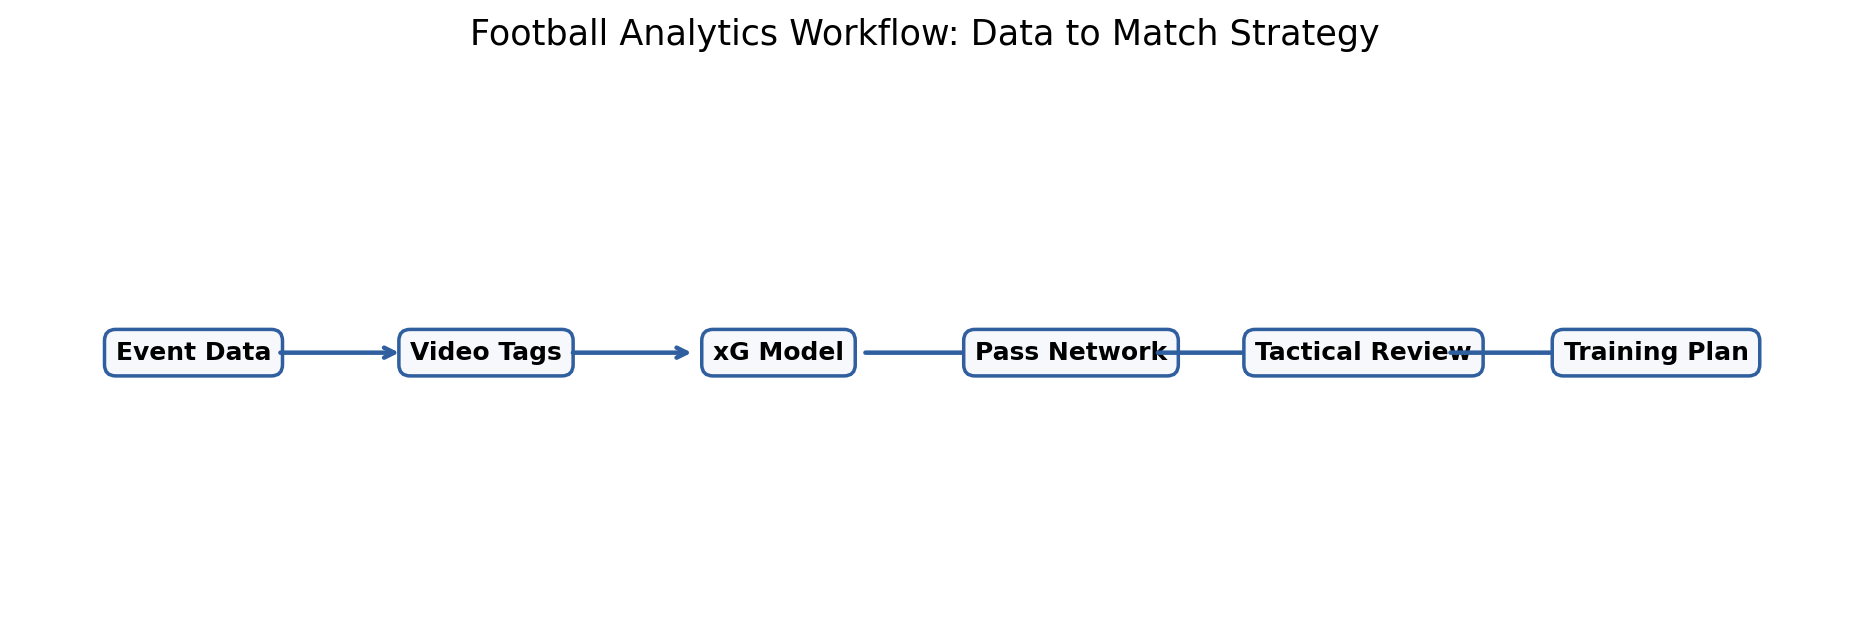
\includegraphics[width=0.9\textwidth]{assets/agent_pipeline_graph.png}
\caption{זרימת החלטה טקטית: מאיסוף אירועים ועד המלצה למאמן.}
\end{figure}

\begin{table}[h]
\centering
\small
\begin{tabular}{p{0.18\linewidth}p{0.25\linewidth}p{0.43\linewidth}}
\toprule
Metric & מה הוא מודד & שימוש טקטי \\
\midrule
xG & איכות בעיטות & לבדוק אם הקבוצה יוצרת מצבים טובים \\
PPDA & עוצמת לחץ & להשוות לחץ גבוה מול לחץ פסיבי \\
Field tilt & שליטה בשליש היריב & לזהות החזקת כדור מסוכנת \\
Progressive passes & קידום כדור & למדוד שבירת קווי הגנה \\
Pass network & קשרים בין שחקנים & לזהות מוקדי בנייה ובידוד שחקנים \\
\bottomrule
\end{tabular}
\normalsize
\caption{השוואה בין מדדים מרכזיים בניתוח כדורגל.}
\end{table}
\begin{equation}
Q = \sum_{i=1}^{n} w_i \cdot s_i
\end{equation}
\section{מעבר דו-כיווני בין עברית לאנגלית}
הטקסט הראשי כתוב בעברית (RTL), ומונחים טכניים נשמרים באנגלית (LTR). לדוגמה, משפט שלם באנגלית:
\begin{english}
The analyst compares xG, PPDA, pass networks, and video clips before recommending a tactical adjustment.
\end{english}
כאן מודגם המעבר התקין בין כיוון הכתיבה מימין-לשמאל לכיוון משמאל-לימין.
\chapter{איסוף נתונים: אירועים, מיקום ווידאו}
\section{Event data: הפעולות שמרכיבות את המשחק}
Event data הוא שכבת הנתונים הנגישה ביותר בכדורגל מקצועני. הוא מתאר פעולות בדידות כגון מסירה, בעיטה, תיקול, חילוץ, דריבל, הרמה או איבוד כדור. לכל פעולה מצורפים בדרך כלל זמן, קבוצה, שחקן, מיקום על המגרש, תוצאה של הפעולה ולעיתים גם מאפיינים נוספים כמו רגל ימין או שמאל, לחץ יריב או סוג המסירה. היתרון הגדול של event data הוא שהוא קל יחסית לאיסוף, ניתוח והצגה. ניתן לבנות ממנו מפות בעיטות, שרשראות מסירות, מדדי יצירת מצבים ופרופילים של שחקנים. החיסרון הוא שהוא מתאר בעיקר את מה שקרה עם הכדור, בעוד שחלק גדול מהכדורגל מתרחש בלי הכדור. אם קשר מושך שני מגנים בתנועה חכמה ומשאיר חלוץ פנוי, ייתכן שהתרומה שלו לא תופיע כאירוע ברור. לכן event data מתאים במיוחד לשאלות על פעולות, אך פחות לשאלות על מבנה, מרחקים וסגירת שטחים. שימוש נכון בו מחייב הגדרות קבועות: מה נחשב לחץ, מה נחשב מסירה קדימה, ומה נחשב מצב מסוכן. בלי עקביות כזו, המודל ילמד רעש במקום כדורגל.

\section{Tracking data: לראות את השחקנים שלא נוגעים בכדור}
Tracking data מוסיף ממד עמוק יותר משום שהוא מתעד את מיקום כל השחקנים והכדור בתדירות גבוהה לאורך המשחק. במקום לשאול רק מי מסר למי, אפשר לשאול אילו מרווחים נפתחו, כמה קומפקטית הייתה ההגנה, האם הקבוצה שמרה על קווי לחץ, ומה היה המרחק בין הבלמים לקשרים. נתונים אלה מאפשרים לבנות מדדים כמו team width, defensive line height, pitch control ו-space occupation. לדוגמה, קבוצה עשויה להחזיק מעט בכדור אך לשלוט במרחבים החשובים אם היא סוגרת נתיבי מסירה ומכריחה את היריבה לשחק לאזורים חסרי ערך. Tracking data גם מאפשר לנתח תנועה ללא כדור: ריצות עומק, פתיחת זוויות, תזמון לחץ וחיפוי. עם זאת, הוא יקר יותר, כבד יותר לעיבוד ורגיש לטעויות כיול. בנוסף, נתוני מיקום בלי הבנה טקטית עלולים להטעות. שחקן שנראה רחוק מהכדור עשוי למלא תפקיד קריטי בסגירת קו מסירה. לכן השימוש הטוב ביותר ב-tracking data הוא שילוב בין חישוב אוטומטי לבין פרשנות מקצועית של המאמן והאנליסט.

\section{וידאו ותיוג אנושי כחוליה מקשרת}
למרות ההתקדמות במדדים אוטומטיים, וידאו נשאר כלי מרכזי משום שהוא מחזיר את הנתון להקשר האנושי. מספר יכול להראות שקבוצה איבדה כדורים רבים באזור מסוים, אך הווידאו מסביר האם האיבודים נבעו מלחץ טוב של היריבה, ממיקום גוף לא נכון, מתזמון תנועה חלש או מהחלטה טכנית של שחקן. תיוג וידאו מאפשר ליצור קטגוריות שמודלים כלליים אינם מזהים היטב: pressing trap, third-man run, underlap, rest defence או overload באגף. כאשר האנליסט בונה ספריית קליפים סביב תובנה מספרית, המאמן יכול להפוך אותה לאימון מעשי. כאן נוצר החיבור החשוב בין AI לבין צוות מקצועי: האלגוריתם מציף דפוס, האדם נותן לו שם ומשמעות, והקבוצה מתרגלת שינוי. תהליך כזה גם מצמצם התנגדות מצד שחקנים, כי קל יותר לקבל נתון כאשר רואים אותו חוזר בווידאו. לכן ניתוח כדורגל טוב אינו מסתפק בטבלה; הוא בונה סיפור ראייתי שמחבר בין מספרים, קליפים והוראות משחק.

לקריאה נוספת בנושאי פרק זה, ראו \cite{langchain_docs}.

\chapter{מדדים טקטיים: לחץ, החזקת כדור ויצירת מצבים}
\section{לחץ ו-PPDA כמדד לסגנון הגנתי}
לחץ הוא אחד הנושאים המרכזיים בכדורגל מודרני, אך קשה למדוד אותו היטב. מדד נפוץ הוא PPDA, כלומר passes allowed per defensive action. באופן כללי, ערך נמוך מצביע על קבוצה שמאפשרת ליריבה פחות מסירות לפני פעולה הגנתית, ולכן עשוי להעיד על לחץ גבוה ואגרסיבי. אבל PPDA לבדו אינו מספיק. קבוצה יכולה לקבל ערך נמוך כי היא לוחצת חכם, או כי היא רצה ללא סדר ומשאירה שטחים מאחור. לכן חשוב לחבר את המדד למיקום הפעולות, לגובה קו ההגנה, למרחקים בין שחקנים ולתוצאה אחרי החילוץ. לחץ איכותי אינו רק ניסיון לחטוף את הכדור; לעיתים המטרה היא לכוון את היריבה לאגף, להכריח מסירה אחורה או למנוע מסירה לקשר אחורי. אנליסט טוב יבדוק האם הלחץ יוצר יתרון ממשי: איבודים באזור מסוכן, בעיטות אחרי חילוץ, או ירידה באיכות ההתקפות של היריבה. כך PPDA הופך מנקודת פתיחה לשיחה מקצועית על מבנה הגנתי.

\section{החזקת כדור איכותית מול החזקת כדור ריקה}
אחוזי החזקת כדור הם אחד הנתונים הישנים והפופולריים ביותר, אך הם גם עלולים להטעות. קבוצה יכולה להחזיק 65 אחוז מהזמן בכדור ועדיין לא לאיים על השער, אם רוב המסירות הן בין הבלמים או באזורים רחוקים. לכן אנליסטים מעדיפים לשאול האם ההחזקה מקדמת את הקבוצה לעמדות טובות. מדדים כמו progressive passes, entries to final third, box entries ו-field tilt עוזרים להבין אם הקבוצה באמת שולטת במרחב המסוכן. החזקת כדור איכותית יוצרת הזזת יריבה, פתיחת קווי מסירה, שינויי צד ותזמון כניסות לרחבה. החזקת כדור ריקה, לעומת זאת, יכולה להיות סימן לכך שהיריבה נוחה, סגורה וממתינה לטעות. גם כאן ההקשר חשוב: מול יריבה חזקה, החזקה זהירה עשויה להיות בחירה נכונה לשליטה בקצב; מול בלוק נמוך היא עלולה להעיד על חוסר יצירתיות. לכן מדדי החזקה חייבים להיקרא יחד עם וידאו, מערך היריבה ומטרת המשחק.

\section{שרשראות התקפה ותרומה של שחקנים}
כדי להבין יצירת מצבים, לא מספיק לספור בישולים ובעיטות. שער נולד לעיתים עשר פעולות לפני המסירה האחרונה: חילוץ, מסירה בין קווים, תנועה מושכת, החלפת צד ודריבל שיוצר יתרון. לכן מודלים מתקדמים בוחנים possession chains ומייחסים ערך לפעולות שמקדמות התקפה. מדדים כמו expected threat, expected possession value או shot contribution מנסים להעריך כיצד פעולה משנה את הסיכוי להגיע למצב איכותי. קשר שמוסר קדימה בין שני שחקנים עשוי לתרום יותר ממוסר המסירה האחרונה הפשוטה, גם אם לא יקבל בישול. מגן שמייצר קבוע יתרון באגף יכול להיות חשוב מאוד גם בלי מספרים נוצצים. גישה זו משנה גם סקאוטינג: במקום לחפש רק שערים ובישולים, אפשר לזהות שחקנים שמקדמים כדור, שוברים קווים או מקבלים החלטות נכונות תחת לחץ. המדדים אינם מבטלים את הצפייה בשחקן, אך הם מצמצמים הטיות ומכוונים את העין למה שבאמת חוזר לאורך זמן.

לקריאה נוספת בנושאי פרק זה, ראו \cite{latex_project}.

\chapter{גרפים ורשתות מסירה: לראות את מבנה הקבוצה}
\section{Pass network כצילום של מבנה התקפי}
Pass network מציג את השחקנים כצמתים ואת המסירות ביניהם כקשרים. גודל הצומת יכול לייצג כמות נגיעות או מעורבות, ועובי הקו יכול לייצג מספר מסירות בין שני שחקנים. גרף כזה אינו מחליף צפייה במשחק, אך הוא נותן תמונה מהירה של מי היו מוקדי המשחק, האם הקבוצה בנתה בעיקר דרך צד אחד, והאם שחקנים מסוימים היו מנותקים. אם הקו בין הבלם לקשר האחורי עבה מאוד, ייתכן שהקבוצה הצליחה לצאת מסודר מהלחץ. אם החלוץ כמעט לא מחובר לרשת, ייתכן שהקבוצה לא מצאה אותו בין הקווים. עם זאת, צריך להיזהר: רשת מסירות ממוצעת יכולה להסתיר שינויים בין מחציות, חילופים או מצב תוצאה. לכן מומלץ לבנות גרפים לפי פרקי זמן, מצבי משחק או אזורי מגרש. כאשר מצמידים גרף כזה לקליפים נבחרים, הוא הופך לכלי מצוין לדיון טקטי עם הצוות.

\section{מפות חום ואזורים מסוכנים}
מפת חום מציגה איפה פעולות התרחשו בתדירות גבוהה, אך הפרשנות שלה תלויה בשאלה המקצועית. מפת נגיעות של מגן יכולה להראות אם הוא נשאר נמוך, תוקף גבוה או נכנס למרכז כמו inverted fullback. מפת בעיטות יכולה לחשוף האם קבוצה מגיעה למצבים מתוך הרחבה או מסתפקת בבעיטות מרחוק. מפת לחץ יכולה להראות האם המלכודת ההגנתית מתרחשת באגף ימין, במרכז או סביב קשר יריב מסוים. אבל מפת חום אינה מודדת איכות לבדה. אזור מלא בפעולות עשוי להיות תוצאה של שליטה יעילה או של תקיעות. לכן אנליסט צריך לשלב בין צפיפות הפעולות לבין ערך הפעולות: האם הפעולות באזור הזה העלו xG, יצרו כניסות לרחבה או עצרו התקפות יריב. שימוש נכון במפות חום עוזר למאמן לענות על שאלות כמו האם הקבוצה מנצלת את האגף החלש, האם הקשרים קרובים מספיק לחלוץ, והאם יש שטחים שלא מכוסים במעבר הגנתי.

\section{גרף כבסיס לשיחה ולא כקישוט}
גרף טוב בכדורגל צריך לענות על שאלה אחת ברורה. אם הוא עמוס מדי, צבעוני מדי או חסר כותרת מקצועית, הוא עלול להפוך לקישוט שמרשים לרגע אך לא משנה החלטה. לכן לפני בניית גרף צריך לשאול מה המאמן צריך להבין: האם הלחץ עובד, האם הקבוצה בונה דרך צד אחד, האם החלוץ מבודד, או האם חילוף שינה את מרכז הכובד. רק אחר כך בוחרים ייצוג מתאים. רשת מסירות מתאימה לקשרים בין שחקנים, מפת חום מתאימה למיקום, גרף קווי מתאים לשינוי לאורך זמן, וטבלה מתאימה להשוואה בין קבוצות או שחקנים. חשוב גם להציג יחידות, מקור נתונים והגבלות. למשל, גרף xG ללא ציון שהפנדלים נכללו או הוצאו עלול להטעות. כאשר גרף נבנה סביב שאלה מקצועית, הוא יוצר שפה משותפת: האנליסט מסביר, המאמן שואל, והשחקן מבין מה צריך לשנות במגרש.

לקריאה נוספת בנושאי פרק זה, ראו \cite{crewai_docs}.

\chapter{AI בסקאוטינג, הכנה ליריבה וניהול משחק}
\section{סקאוטינג מבוסס פרופילים ולא רק מספרים}
סקאוטינג מודרני משתמש בנתונים כדי לצמצם מרחב חיפוש גדול. במקום לצפות באלפי שחקנים באופן ידני, המועדון יכול להגדיר פרופיל: קשר שמקדם כדור תחת לחץ, מגן שמייצר מסירות לרחבה, בלם שמגן בשטח פתוח או חלוץ שמגיע להרבה מצבים איכותיים. המודל מסנן מועמדים לפי מדדים, גיל, ליגה, תפקיד ועלות משוערת. אבל זה רק השלב הראשון. לאחר מכן צריך לבדוק התאמה טקטית, איכות טכנית, אופי, פציעות, הסתגלות לליגה וסביבה חברתית. מספרים יכולים לחשוף שחקן שאינו מוכר, אך הם לא מספרים את כל הסיפור. גם חשוב לתקן הקשר: שחקן בליגה חלשה או בקבוצה דומיננטית עשוי להיראות טוב במדדים מסוימים, אך להתמודד עם דרישות שונות לגמרי בקבוצה אחרת. לכן AI בסקאוטינג הוא כלי להרחבת ראייה ולהפחתת הטיות, לא תחליף לסקאוט מקצועי. ההחלטה הטובה ביותר נוצרת כאשר מודל, וידאו, דוח אנושי ואסטרטגיית מועדון נפגשים.

\section{הכנה ליריבה: זיהוי דפוסים חוזרים}
לפני משחק, צוות מקצועי מנסה להבין מה היריבה עושה שוב ושוב: איך היא מתחילה התקפות, איפה היא מאבדת כדור, מי השחקן שמקבל בין הקווים, ואיפה היא פגיעה במעברים. AI יכול לסייע בזיהוי דפוסים אלה על ידי חיפוש אוטומטי בנתוני משחקים קודמים. למשל, המודל יכול לאתר שרשראות שבהן היריבה יוצאת דרך הבלם השמאלי ואז מחפשת מסירה אל הקשר האחורי, או מצבים שבהם המגן הימני עולה ומשאיר שטח מאחור. לאחר הזיהוי, האנליסט בונה קליפים והמאמן מתרגם אותם לתוכנית: ללחוץ על שחקן מסוים, לסגור קו מסירה, או לתקוף אזור חלש. היתרון הוא מהירות ועקביות; החיסרון הוא סכנת עודף מידע. שחקנים אינם יכולים לזכור עשרים דפוסים. לכן תוצר טוב להכנה ליריבה צריך להיות קצר, חד ומעשי: שלוש נקודות מפתח, שני קליפים לכל נקודה, והוראה ברורה להתנהגות במגרש.

\section{ניהול משחק בזמן אמת}
בזמן משחק, החלטות מתקבלות תחת לחץ עצום ומידע חלקי. האם להחליף שחקן עייף, לשנות מערך, להוריד קו, ללחוץ גבוה יותר או להכניס חלוץ נוסף? מערכות נתונים בזמן אמת יכולות לספק סימנים: ירידה במהירות ספרינט, איבודי כדור באזור מסוכן, שינוי במרכז הכובד של היריבה או ירידה בכמות הכניסות לרחבה. אבל יש גבול למה שמודל יכול לדעת. הוא לא תמיד מבין פציעה קטנה, מצב רגשי, הוראה טקטית שניתנה בדקה קודמת או שיקול של חדר הלבשה. לכן AI בזמן אמת צריך להיות מערכת התראה, לא טייס אוטומטי. תפקידו להעלות שאלות בזמן: האם הקשר המרכזי כבר לא סוגר שטחים, האם האגף השמאלי נחשף, האם היריבה מצליחה לצאת מהלחץ באותה תבנית. המאמן מחליט, אבל מקבל איתותים מבוססי נתונים שמקטינים עיוורון. כך הטכנולוגיה תומכת בניהול המשחק בלי לפגוע באחריות המקצועית.

לקריאה נוספת בנושאי פרק זה, ראו \cite{langchain_docs}.

\chapter{אתיקה, מגבלות והעתיד של אנליטיקה בכדורגל}
\section{הטיות במדדים ובמודלים}
כל מודל נבנה מתוך נתונים, וכל נתון נוצר מתוך החלטות אנושיות. לכן גם אנליטיקה בכדורגל עלולה לשאת הטיות. אם מודל סקאוטינג מאומן בעיקר על ליגות עשירות, הוא עשוי להעדיף שחקנים מסגנון מסוים ולהחמיץ כישרונות מסביבות אחרות. אם מדד מעריך מסירות קדימה אך מתעלם מתנועה ללא כדור, הוא עלול להמעיט בערך שחקנים שמפנים שטחים. אם מודל xG אינו כולל לחץ איכותי או מיקום שוער, הוא עלול להעריך מצבים באופן גס מדי. בנוסף, מדדים יכולים להשפיע על התנהגות: שחקן שיודע שמודדים אותו לפי בעיטות עשוי לבחור בעיטה במקום מסירה טובה יותר. לכן חשוב לראות מדדים כמכשירים עם מגבלות, לא כשפה ניטרלית לחלוטין. מועדון אחראי בודק את המודלים שלו, משווה אותם לווידאו, ומאפשר לאנשי מקצוע לערער על מסקנות. ביקורת כזו אינה חולשה; היא תנאי לכך שנתונים ישרתו כדורגל טוב יותר.

\section{פרטיות, עומס ומעקב אחרי שחקנים}
ככל שמועדונים אוספים יותר נתונים, עולה שאלה אתית: איפה עובר הגבול בין שיפור ביצועים לבין מעקב מוגזם. נתוני GPS, עומסים פיזיים, דופק, שינה, התאוששות ולעיתים גם מידע רפואי יכולים לעזור למנוע פציעות ולתכנן אימונים. אך הם גם מידע רגיש מאוד על גוף האדם. שחקן צריך לדעת אילו נתונים נאספים, מי רואה אותם, כמה זמן הם נשמרים וכיצד משתמשים בהם בחוזים, החלטות מקצועיות או העברות. אמון הוא תנאי מרכזי. אם השחקנים ירגישו שהנתונים משמשים נגדם, הם יסתירו מידע או יתנגדו למערכת. לכן שימוש אחראי דורש שקיפות, הרשאות מוגבלות, הפרדה בין צוות רפואי לצוות מקצועי במידע רגיש, והסבר ברור על מטרות המדידה. אנליטיקה טובה אינה רק מדויקת טכנית; היא גם הוגנת ביחסים בין מועדון לשחקן.

\section{העתיד: שיתוף פעולה בין אדם למודל}
העתיד של אנליטיקה בכדורגל אינו מאמן רובוטי שמקבל החלטות לבדו, אלא שיתוף פעולה עמוק יותר בין אדם למודל. מודלים יהיו טובים יותר בזיהוי דפוסים, בהמלצת קליפים, בהשוואת שחקנים ובהערכת סיכונים. במקביל, מאמנים ואנליסטים יצטרכו לשאול שאלות טובות יותר, להבין מגבלות ולהסביר תובנות בשפה פשוטה לשחקנים. היתרון התחרותי לא יהיה רק למועדון שקונה את המערכת היקרה ביותר, אלא לזה שמטמיע אותה בתוך תרבות עבודה בריאה: שאלות ברורות, בדיקת השערות, חיבור לווידאו, משוב מהשחקנים ולמידה מתמשכת. כדורגל יישאר משחק של החלטות אנושיות, לחץ, יצירתיות ואומץ. הנתונים יכולים להאיר את המגרש מזווית חדשה, אך הם אינם מחליפים את המגרש עצמו. כאשר משתמשים בהם בענווה ובדיוק, הם מאפשרים למועדון לראות יותר, לטעות פחות, ולהפוך רעיון טקטי לתוכנית עבודה מדידה.

לקריאה נוספת בנושאי פרק זה, ראו \cite{latex_project}.

\chapter{תוכנית הטמעה מעשית במועדון כדורגל}
\section{להתחיל משאלות מקצועיות ולא ממערכת יקרה}
הטעות הנפוצה ביותר בהטמעת אנליטיקה בכדורגל היא להתחיל מהטכנולוגיה במקום מהבעיה המקצועית. מועדון יכול לרכוש מערכת וידאו מתקדמת, מאגר נתונים רחב ולוח מחוונים יפה, ועדיין לא לשנות אף החלטה אם אין שאלה ברורה שמובילה את העבודה. לכן הצעד הראשון צריך להיות סדנה קצרה עם המאמן, עוזרי המאמן, מנהל הספורט והאנליסט: אילו החלטות חוזרות הכי משפיעות על הקבוצה? האם הבעיה היא יצירת מצבים מול בלוק נמוך, הגנה במעברים, בחירת שחקנים להרכב, עומסים באימונים או סקאוטינג לעמדה מסוימת. לכל שאלה כזו מגדירים מדד מוביל, מקור נתונים, תדירות בדיקה ותוצר צפוי. למשל, אם המטרה היא לשפר לחץ גבוה, התוצר אינו רק מספר PPDA אלא דוח שבועי שמראה איפה הלחץ מתחיל, אילו שחקנים מאחרים לסגור, ומה קורה בחמש השניות אחרי חילוץ. אם המטרה היא סקאוטינג, התוצר הוא shortlist עם קליפים ודירוג התאמה, לא גיליון מספרים אינסופי. גישה כזו מונעת בזבוז ומחברת את האנליטיקה לשפה של אנשי המקצוע. הטכנולוגיה נכנסת רק לאחר שהמועדון יודע מה הוא רוצה למדוד, מי ישתמש בתובנה, ואיזו החלטה היא אמורה לשפר.

\section{שגרת עבודה שבועית בין אנליסט למאמן}
כדי שאנליטיקה תהפוך לחלק מהקבוצה, היא צריכה להיכנס לשגרה ולא להישאר פרויקט צדדי. שבוע עבודה טיפוסי יכול להתחיל ביום שאחרי המשחק עם דוח post-match קצר: שלוש תובנות מספריות, שלושה קליפים תומכים ושאלה אחת להמשך. באמצע השבוע האנליסט מכין דוח יריבה ממוקד, שבו מוצגים דפוסי בנייה, נקודות חולשה, מצבי נייחים ומדדים מרכזיים כמו xG against, אזורי איבוד ונטייה ללחץ. יום לפני המשחק, התוצר לשחקנים צריך להיות מצומצם הרבה יותר: מעט קליפים, הוראות פשוטות ומושגים שחוזרים באימון. אחרי המשחק, חוזרים לאותן שאלות ובודקים אם התוכנית עבדה. החשיבות של השגרה היא שהיא יוצרת אמון. המאמן יודע מתי יקבל מידע, האנליסט יודע איזה עומק נדרש, והשחקנים לא מוצפים במספרים. בנוסף, שגרה מאפשרת למועדון ללמוד לאורך זמן: האם המדדים שנבחרו באמת מנבאים ביצועים, האם תובנות מסוימות חוזרות, והאם האימון משנה את הנתונים. בלי מחזור קבוע של שאלה, מדידה, וידאו, אימון ובדיקה חוזרת, אנליטיקה נשארת מצגת יפה. עם מחזור כזה, היא הופכת לכלי ניהולי שמחבר בין תכנון שבועי לבין ביצוע במגרש.

\section{מדדי הצלחה לפרויקט אנליטיקה}
פרויקט אנליטיקה צריך להימדד גם לפי איכות העבודה הפנימית ולא רק לפי תוצאות בטבלה, משום שתוצאות משחק מושפעות מגורמים רבים כמו פציעות, מזל, איכות יריבה ושיפוט. לכן מועדון צריך להגדיר מדדי הצלחה תפעוליים. הראשון הוא adoption: האם המאמן משתמש בדוחות, האם עוזרי המאמן מבקשים ניתוחים, והאם שחקנים מזהים את המושגים באימון. השני הוא decision impact: כמה החלטות בפועל הושפעו מהנתונים, כמו שינוי תרגיל אימון, בחירת שחקן, התאמה ליריבה או שינוי הוראה במצבים נייחים. השלישי הוא speed: כמה זמן לוקח להפוך משחק גולמי לדוח שימושי. הרביעי הוא accuracy and review: האם תובנות שניתנו לפני משחק נבדקו לאחריו, והאם המועדון למד מטעויות. החמישי הוא communication quality: האם התוצר ברור לאדם שאינו אנליסט, או שהוא דורש פענוח טכני ארוך. לצד המדדים הפנימיים אפשר לעקוב גם אחרי מדדים מקצועיים כמו איכות מצבים, ירידה באיבודים מסוכנים, שיפור במניעת בעיטות או עלייה בכמות כניסות לרחבה. המטרה אינה להוכיח שהמודל תמיד צדק, אלא לבנות מערכת למידה. כאשר המועדון מודד את האנליטיקה עצמה, הוא משפר בהדרגה את השאלות, את הנתונים ואת התקשורת בין כל בעלי התפקידים. חשוב גם לקבוע נקודת ביקורת חודשית שבה בוחנים אילו דוחות באמת נקראו, אילו קליפים נכנסו לאימון, ואילו מדדים ננטשו כי לא תרמו להחלטה. ביקורת כזו מונעת מצב שבו המחלקה האנליטית מייצרת עבודה מרשימה אך מנותקת. היא מעודדת פשטות, אחריות ושיפור מתמשך, ומזכירה שהמטרה הסופית אינה להיות מתקדם טכנולוגית אלא לשחק כדורגל ברור, חכם ויעיל יותר. בנוסף, מומלץ לשמור יומן החלטות קצר: מה הייתה ההשערה, איזה נתון תמך בה, איזו פעולה בוצעה, ומה למדנו לאחר המשחק. יומן כזה יוצר זיכרון ארגוני, מפחית ויכוחים בדיעבד, ומאפשר למועדון להשוות בין תחושות לבין ראיות לאורך עונה שלמה. בסוף כל חודש אפשר לבחור החלטה אחת שהצליחה והחלטה אחת שנכשלה, לנתח אותן יחד עם הצוות, ולהפוך את המסקנות לכללי עבודה פשוטים. כך האנליטיקה נעשית תרבות למידה ולא רק דוח טכני. תהליך עקבי כזה גם מקל על אנשי צוות חדשים להבין במהירות את סגנון המועדון ואת שפת ההחלטות שלו.

לקריאה נוספת בנושאי פרק זה, ראו \cite{crewai_docs}.

\nocite{*}
\printbibliography
\end{document}